\chapter{Background}
\label{cha:background}

In this chapter, we introduce the necessary logical and compiler background concepts required for the understanding of the material presented in this thesis. In Section~\ref{sec:lambda_calc}, we review some of the mathematical background useful for understanding our optimisations. In Section~\ref{sec:agda_compiler}, we give an introduction to the Agda compiler. Finally, in Section~\ref{sec:background_conclusion}, we conclude with a summary of the core concepts and describe where they are used throughout the remainder of the thesis.

\section{Lambda Calculus}
\label{sec:lambda_calc}

Lambda calculus (or $\lambda$-calculus) is a formal system for representing computational logic in terms of function abstractions and applications using variable binding and substitution. It warrants our understanding because concepts surrounding the Agda programming language and its compilation are inspired by, and can be elegantly explained by, the framework of the lambda calculi.\cite{fokkinga1987} In fact, the namesake of the default Agda GHC backend, MAlonzo, is Alonzo Church, the mathematician who first developed the lambda calculus.\cite{fokkinga1987}

\subsection{Pure $\lambda$-Calculus}

In a pure $\lambda$-calculus, terms are built inductively from only variables, $\lambda$-abstractions and applications, as in Figure~\ref{fig:lambda_calc}.\cite{kozen1997}

\begin{figure}
\begin{align*}
t ::=~& x               & \text{variable}\\
    |~& \lambda x . t   & \text{abstraction}\\
    |~& t~t             & \text{application}
\end{align*}
\caption{Grammar of a pure lambda calculus.}
\label{fig:lambda_calc}
\end{figure}

\subsection{De Bruijn Index Notation}

In order to eliminate the need for named variables in $\lambda$-calculus notation, de Bruijn indexed notation is used to represent bound terms (variables) with natural numbers. In any term, the positive integer $n$ refers to the $n$th surrounding $\lambda$ binder.\cite{debruijn1972} In other words, the number is an index indicating the number of variable binders (or $\lambda$-abstractions) in scope between itself and the binder for the variable being referenced. The grammar of a de Bruijn-indexed lambda calculus can be seen in Figure~\ref{fig:db_lambda_calc}. See Figure~\ref{fig:db_example} for an illustration where the variable bindings and indices are coloured to indicate matches and the references are shown with arrows.

\begin{figure}
\centering
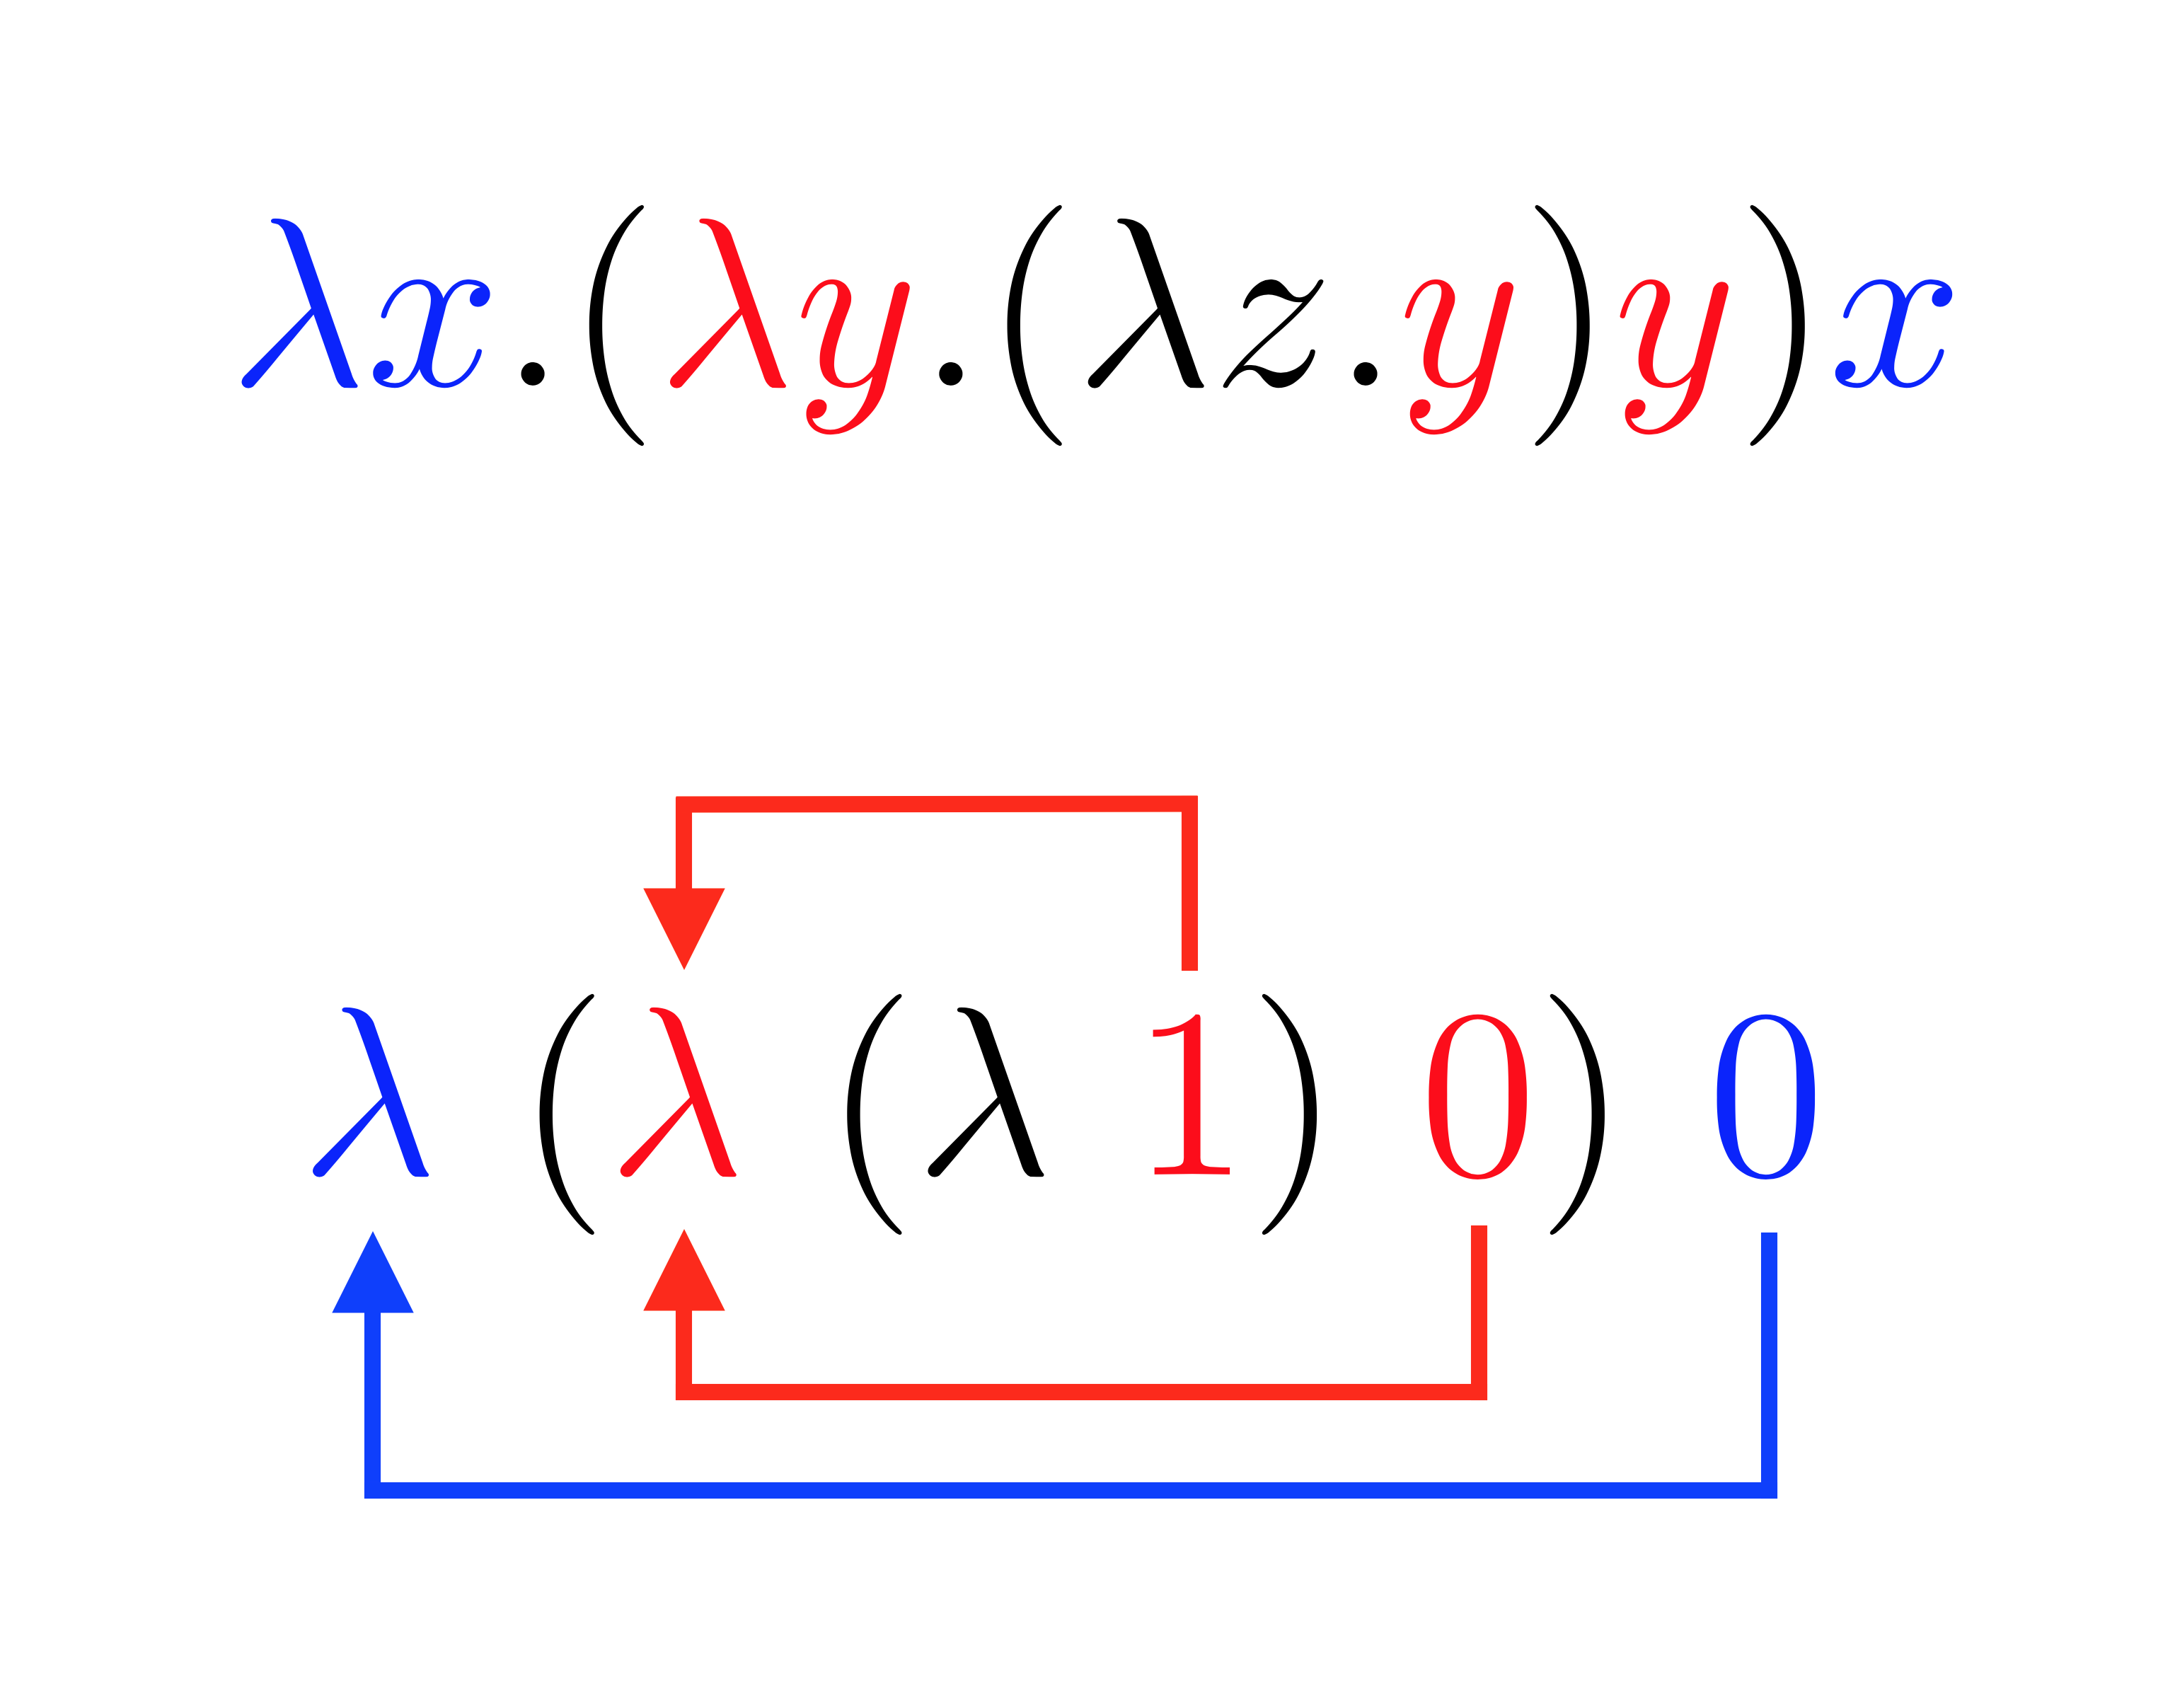
\includegraphics[width=8cm]{Figures/DeBruijnIndex}
\caption{Example of a de Bruijn indexed $\lambda$-calculus expression.\cite{chaudhuri2009}}
\label{fig:db_example}
\end{figure}

\edcomm{NP}{Better if graphic emphasizes that in different scope locations, different numbers point to the same bound variable.}

\begin{figure}
\begin{align*}
t ::=~& \mathbb{N}      & \text{variable}\\
    |~& \lambda~t       & \text{abstraction}\\
    |~& t~t             & \text{application}
\end{align*}
\caption{Grammar of a pure lambda calculus.}
\label{fig:db_lambda_calc}
\end{figure}

The internal representation of Agda code in the compiler is based on a de Bruijn indexed $\lambda$-calculus.

\subsection{$\lambda\sigma$-Calculus}

In order to perform the desired optimisations on the abstract syntax tree, we must be able to perform substitutions on terms. Treating the abstract syntax tree structure as a specialized $\lambda$-calculus, we can implement substitution as a function on terms.

Because our terms are built on de Bruijn indexed variables, we use the explicit substitution of a $\lambda\sigma$-calculus as a reference for understanding correct substitution on terms in the context of local variables bound by incrementing indices. The $\lambda\sigma$-calculus is a refinement of the $\lambda$-calculus where substitutions are manipulated explicitly, and substitution application is a term constructor rather than a meta-level notation.\cite{abadi1991}

\subsection{Substitution}

Take then, for instance, a simple case of the classical application of the $\beta$-rule (See Figure~\ref{eq:beta_rule}). Beta reduction is the process of simplifying an application of a function to the resulting substituted term. However, in order to $\beta$-reduce $(\lambda a)b$, we must not only substitute $b$ into the appropriate occurrences in $a$. As the $\lambda$ binding disappears, we must also decrement all remaining free indices in $a$. This adapted form of the $\beta$-rule can be represented by the infinite substitution showin in Figure~\ref{eq:beta_rule2}).\cite{abadi1991}

\begin{figure}
\begin{equation*}
(\lambda x.t)s \to_{\beta} t[x := s]
\end{equation*}
\caption{The classical $\beta$-reduction rule.}
\label{eq:beta_rule}
\end{figure}

\begin{figure}
\begin{equation*}
(\lambda t)s \to_{\beta} t[1 := s, 2 := 1, 3 := 2, ...]
\end{equation*}
\caption{The modified $\beta$-reduction rule for de Bruijn notation.}
\label{eq:beta_rule2}
\end{figure}

However, the substitution in this adapted rule must be evaluated carefully to produce a correct result. Consider if the term $t$ contains another $\lambda$ binding. As the substitution is applied to that nested $\lambda$ term, occurences of $1$ should not be replaced with $s$, because occurrences of $1$ refer to the nested $\lambda$ term's bound variable. Instead, occurrences of $2$ should be replaced with $s$; likewise, occurrences of $3$ should be replaced by $2$, and so on. We thus ``shift'' the substitution.\cite{abadi1991}

It is also important when applying substitutions to $\lambda$ terms that we avoid the unintended capture of free variables in our terms being substituted in. Imagine again the nested $\lambda$ term, with occurences of $2$ being replaced with $s$. Occurences of $1$ in $s$ must be replaced with $2$, else the nested $\lambda$ binder will capture the index. We this ``lift'' the indices of $s$. These two caveats result in the substitution rule in Figure~\ref{eq:debruijn_sub}.\cite{abadi1991}

\begin{figure}
\begin{equation*}
(\lambda t)[1 := s, 2 := 1, ...] = \lambda t[2 := s[1 := 2, 2 := 3, ...], 3 := 2, ...]
\end{equation*}
\caption{The substitution rule for de Bruijn indexed lambda terms.}
\label{eq:debruijn_sub}
\end{figure}

Recognizing the required index ``shifting'' and ``lifting'' in the Figure~\ref{eq:debruijn_sub} substitution rule should suffice as background for understanding the variable manipulation performed in our optimisation.

\section{Agda Compiler}
\label{sec:agda_compiler}

The Agda programming language's first and most-used backend is MAlonzo, or more generically, the GHC backend.\cite{benke2007} Given an Adga module containig a \AgdaFunction{main} function\footnote{An Agda module without a main file can be compiled with \texttt{-{}-no-main}.}, the Agda \texttt{-{}-compile} option will compile the program using the GHC backend by default, which translates an Agda program into Haskell source. The generated Haskell source can then be automatically or manually (with \texttt{-{}-ghc-dont-call-ghc}) compiled to an executable program via GHC.\cite{agdadocs} % http://agda.readthedocs.io/en/latest/tools/compilers.html

There are several stages of translation and compilation in this process. The transition of primary interest for our optimisations is the conversion of compiled clauses to a ``treeless'' syntax. This translations occurs after Agda type-checking but before Haskell source is generated. Most Agda optimisations occur as alterations to the treeless terms.

Agda functions begin as a type\footnote{It is worth noting that type inference is an undecidable problem for definitions with dependent types, so type signatures must be provided in many cases, and by convention, should always be provided.} and a definition. Functions on datatypes can be defined by pattern matching on the constructors of that datatype, describing a structurally recursive function.\cite{agdawiki} % http://wiki.portal.chalmers.se/agda/agda.php?n=Docs.DatatypeAndFunctionDefinitions
This should sound familiar to users of functional programming languages like Haskell. Unlike Haskell, however, Agda does not permit partial functions. Therefore, functions defined by pattern matching must not exclude any possible cases from the pattern matching clauses.\cite{agdawiki} % http://wiki.portal.chalmers.se/agda/pmwiki.php?n=ReferenceManual.Totality#Coveragechecking}
Because function definitions in Agda are written as a series of one or more pattern matching clauses on possible variable inputs, we can construct an equivalent definition via case tree.\cite{agdawiki} % http://wiki.portal.chalmers.se/agda/agda.php?n=Docs.PatternMatching
Once coverage checking and type checking is completed, pattern matching can be translated into case trees by successively splitting on each variable.\cite{agdahackage} % https://hackage.haskell.org/package/Agda-2.5.2/docs/Agda-TypeChecking-CompiledClause.html
Compiled clauses are the first stage of compilation and they are, simply put, case trees.

Take for example the simple \AgdaFunction{not} function on booleans in Figure~\ref{code:not_agda}. The compiled clauses of \AgdaFunction{not} are shown in Figure~\ref{code:not_cc}, and the treeless syntax of \AgdaFunction{not} is shown in Figure~\ref{code:not_tterm}.

\input{Figures/Agda/latex/Not}

The treeless syntax is the input to the compiler backend of Agda. It's a high-level internal syntax, the name for which is derived from its use of case expressions instead of case trees. The other notable difference between compiled clauses and treeless syntax is the absence of datatypes and constructors.\cite{agdahackage} % https://hackage.haskell.org/package/Agda-2.5.2/docs/Agda-Syntax-Treeless.html
\edcomm{NP}{Why?}

\subsubsection{Treeless Syntax}

This treeless syntax is constructed from the \lstinline{TTerm}s (\textbf{T}reless \textbf{Terms}) data type and is the representation of the abstract syntax tree that we will refer to most frequently. It can be reasoned about as a lambda calculus with all local variable represented as de Bruijn indices. A listing of \lstinline{TTerm} constructors is shown in Figure~\ref{code:TTerm}.

In this section we examine the constructors of \lstinline{TTerm}s one-by-one.\cite{agdahackage}

\edcomm{NP}{Read about how sharing is lost with substitution in the agda mailing list: \url{https://lists.chalmers.se/pipermail/agda/2017/009379.html}}

\begin{figure}
\begin{lstlisting}[style=blockhaskell]
type Args = [TTerm]

data TTerm = TVar Nat
           | TPrim TPrim
           | TDef QName
           | TApp TTerm Args
           | TLam TTerm
           | TLit Literal
           | TCon QName
           | TLet TTerm TTerm
           | TCase Nat CaseType TTerm [TAlt]
           | TUnit
           | TSort
           | TErased
           | TError TError

data TAlt = TACon QName Nat TTerm
          | TAGuard TTerm TTerm
          | TALit Literal TTerm
\end{lstlisting}
\caption{\lstinline{TTerm} and \lstinline{TAlt} datatype definitions.}
\label{code:TTerm}
\end{figure}

A \textbf{\lstinline{TVar}} is a de Bruijn indexed variable term.

A \textbf{\lstinline{TPrim}} is a compiler-related primitive, such as addition, subtraction and equality on some primitive types.

A \textbf{\lstinline{TDef}} is a qualified name identifying a function or datatype definition \edcomm{NP}{confirm}

A \textbf{\lstinline{TApp}} is a \lstinline{TTerm} applied to a list of arguments, where each argument is itself a \lstinline{TTerm}.

A \textbf{\lstinline{TLam}} % TTerm

A \textbf{\lstinline{TLit}} % Literal

A \textbf{\lstinline{TCon}} % QName

A \textbf{\lstinline{TLet}} introduces a new local term binding in a term body.

A \textbf{\lstinline{TCase}} is a case expression on a case scrutinee (always a de Bruijn indexed variable), a case type, a default value and a list of alternatives.

The case alternatives, \textbf{\lstinline{TAlt}}s, may be constructed from:
\begin{itemize}
\item a \lstinline{TACon}, which matches on a constructor of a given qualified name, binding the appropriate number of pattern variables to the body term if a match is made. Note that a \lstinline{TCase}'s list of \lstinline{Args} must have unique qualified names for each \lstinline{TACon}.
\item a \lstinline{TAGuard}, which matches on a boolean guard and binds no variables if matched against.
\item a \lstinline{TALit}, which matches on a literal term.
\end{itemize}

A \textbf{\lstinline{TUnit}} is used for levels. \edcomm{NP}{what does that mean}

A \textbf{\lstinline{TSort}}

A \textbf{\lstinline{TErased}}

A \textbf{\lstinline{TError}} is used to indicate a runtime error.

\edcomm{NP}{Either before or after compiler section. Discuss Agda module system and its translation. Arguments inheited from all enclosing modules.}

\section{Conclusion}
\label{sec:background_conclusion}

TODO
